
\chapter{Single Tweet's Creditability Scoring Model} % (fold)
\label{cha:single_tweet_creditbility_scoring_model}
Most of the pervious researches are focusing on event level rumors and claims taht the task of classification for individual tweet is not reliable \cite{liu2015real} \cite{ma2015detect} \cite{zhao2015enquiring}, because a single tweet is to short to contains engough features. But Carlos Castillo designed a single tweet's creditability rank system Tweetcred \cite{gupta2014tweetcred}. So we think it is still enable to build up a single tweet creditability model. And we were inspired by the (wenxian) work that we may use nn() without handcrafted features to build up the single tweet's creditability model which in later experiments outputs a better performance.   
\section{Single Tweet's Creditability Model with handcrafted features} % (fold)
First we follow Castillo's \cite{gupta2014tweetcred} idea to implement a single tweet's creditability model with handcrafted features and we test it with decision trees, decision forest and SVM. But the performance of each model are not good enough. 

\subsection{Features}
We use a collection of features major from  Castillo's Tweetcred system\cite{gupta2014tweetcred} totally 27 features in table \ref{tab:single_features}. These features can be extracted directly from Twitter interface without third part website. 
\subsubsection{Text Features}
The Text features capture the content of the text of the tweets. There are 16 Text features. 
\textbf{Sentiment Features} are included in text features.
We used the python natural language Toolkit (nlTK) \footnote{http://www.nltk.org/} to analyze the tweets' sentiment and extract the features: the NumPositiveWords, NumNegativeWords and Polarityscores. Polarity scores is a float for sentiment strength of one tweet\footnote{http://www.nltk.org/api/nltk.sentiment.html} $Polarity\_scores = \frac {1}{N}    \sum_{0}^{n} {Polarity(token_n)}$.

\subsubsection{User Features} We selected total 5 features of the poster. These features are extracted directly from the twitter interface as in figure \ref{fig:UserSample}. ReputationScore is defined as the ratio between \#Friends over \# Followers. $ReputationScore = \frac {\#Friends }{\#Friends +\#Followers}$.
\begin{figure}[!h]
\centering
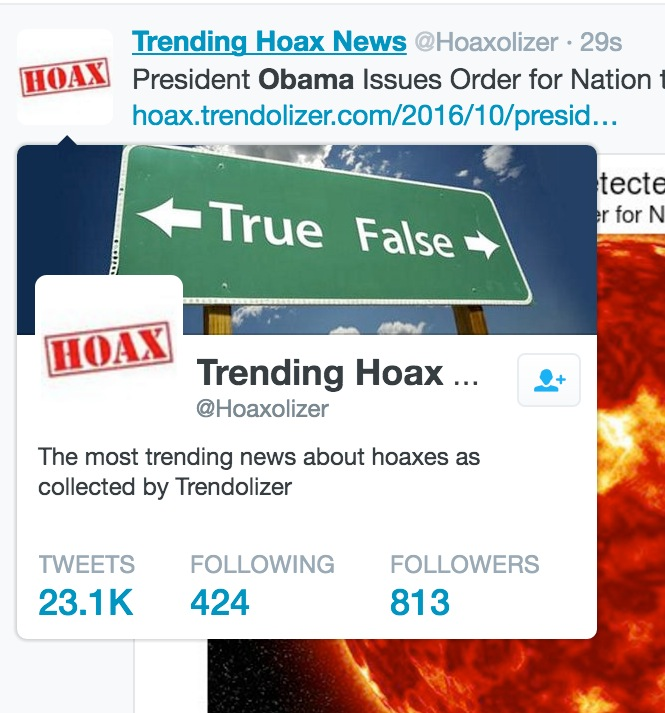
\includegraphics[width=0.55\columnwidth]{images/UserSample.png}
\caption{Sample of Users' Information on Twitter Interface}
\label{fig:UserSample}
\end{figure}

\subsubsection{Twitter Features} Twitter Features are the features of twitter's special functions. It includes Hashtag, Mention, Number of URLs, Number of retweets and whether this tweet is retweet (contains RT as keywords or \emph{"QuoteTweet-innerContainer u-cf js-permalink js-media-container"} as the CSS class of the tweet in html).


\begin{table*}[!h]
\small
\centering
\scalebox{0.8}{
 \begin{tabular}{@{}lllllll@{}}
 \toprule
 \textbf{Category} & \textbf{Feature} & \textbf{Description}\\ \midrule
 Twitter Features& Hashtag & Whether the tweet contains \#hashtag\\
 		& Mention & Whether the tweet mentions others @user\\
 		& NumUrls & \# url in the tweet \\
 		& Retweets & How many times this tweet has been retweeted \\ 
 		& IsRetweet & Whether this tweet is retweeted from others\\
\midrule
 Text Features & LengthOfTweet & The length of tweet\\
    & NumOfChar & \# of individual characters \\
   & Capital &  Fraction of characters in Uppercase \\
   & Smile & Whether this tweet contains :->, :-), ;->, ;-)\\
   & Sad & Whether this tweet contains :-<, :-(, ;->, ;-(\\
   & NumPositiveWords & \# of positive words\\
   & NumNegativeWords & \# of negative words\\
   & PolarityScores & polarity scores of the Tweet\\
   & Via & Whether this tweet contains via\\
   & Stock & Whether this tweet contains \$ \\
   & Question & Whether this tweet contains ? \\
   & Exclamation & Whether this tweet contains ! \\
   & QuestionExclamation & Whether this tweet contains multi Question or Exclamation mark \\ 
   & I & Whether this tweet contains  first pronoun like I, my, mine, we, our   \\
   & You & Whether this tweet contains second pronoun like U, you, your, yours \\ 
   & HeShe & Whether this tweet contains third pronoun like he, she, they, his, etc. \\\midrule
   User Features & UserFollowers  & \# of followers\\
 	& UserFriends  & \# of friends\\
 	& UserTweets  & \# of tweets which are posted by this user\\
 	& UserDescription  & Whether this user has description\\
 	& UserVerified  & Whether this user is a verified user\\
 	& UserReputationScore & Ratio between \#Friends over (\# Followers + \#Friends)\\
 \bottomrule
 \end{tabular}}
 \caption{Features for Single Tweet's Creditability Scoring Model}
 \label{tab:single_features}
\end{table*}
 \newpage

\subsection{Classification Methods}
Most of existing researches use SVM, Random Forest and DT. We test our data also with these 3 models.  We implement these 3 model with scikit-learn library\footnote{scikit-learn.org/}. We shuffled the 260 events and split them into 10 subset, we uses them for 10 times cross-validation. We show the parameters after optimization for each model them in table \ref{tab:single_model_para}.

\begin{table*}[!h]
 \centering
\scalebox{0.8}{
 \begin{tabular}{@{}lllllll@{}}
 \toprule
 \textbf{Model} & \textbf{Parameters} & \textbf{Value} \\ \midrule
 Random Forest & Number of Trees & 200\\ \midrule
 SVM & kernel  & radial basis function\\
 	& penalty parameter of the error term  & 2.0\\
 	& gamma  & $\frac{1}{27}$\\ \midrule
 Decision Trees & criterion & gini \\ \bottomrule
 \end{tabular}}
 \caption{Parameters of Classification models}
 \label{tab:single_model_para}
\end{table*}

 We show the results in the table \ref{tab:single_result}. The  best model with the highest accuracy is RF, but it reaches only 64.87\% and the other two models are even worse, so it is clear to see with manually handcrafted features, one single tweet is difficulty to be classified.  
 \begin{table*}[!h]
 \centering
\scalebox{1.1}{
 \begin{tabular}{@{}lllllll@{}}
 \toprule
 \textbf{Model} & \textbf{Accuracy} \\ \midrule
 Random Forest & \textbf{0.6487 }\\
 SVM &  0.5802\\
 Decision Trees &  0.5774\\ \bottomrule
 \end{tabular}}
 \caption{Prediction Accuracy of Different Single Tweet's Creditability Scoring Models}
 \label{tab:single_result}
\end{table*}

 And we rank the features using the features importance which we mentioned in section \ref{random_forest}, showing in table \ref{tab:Features_Importance}. The best feature is polarity scores of sentiment. It means that there is a big bias between the rumors tweets and the tweets real events. It was mentioned by previous work \cite{allport1947psychology} where he gathered a large rumors collection during WW2 which are printed in the Boston Heralds Rumor Clinic. He summarized rumors as several types:  pipe-dream, fear and aggression. The most researches believe that rumors mostly contain negative sentiment and polarity \cite{sunstein2014rumors}\cite{kwon2013aspects}. In our study average polarity score of news event is -0.066 and average polarity score of rumors is -0.1393, it means that rumors contain more negative sentiment. 
 
 And we usually think the verified users may have less possibility to be involved in the rumors' spreading, but the result shows that the verified users may be not really trustful like we thought. And "IsReweet" feature is neither a good feature which means the probability of people retweeting the rumors or true events are similar.
 
  
 

\begin{table*}[!h]
 \centering
\scalebox{1}{
\begin{tabular}{@{}lllllll@{}}
\toprule
\textbf{Feature} & \textbf{Feature Importance} \\ \midrule
PolarityScores	&	0.1460686474\\
Capital	&	0.09638447209\\
LengthOfTweet  &	0.09283739724\\
UserTweets  &	0.08750049577 \\
UserFriends  &	0.08065591431 \\
UserReputationScore  &	0.08002109553 \\
UserFollowers   &	0.07938657292 \\
NumOfChar	&	0.07659755102\\
Stock	&	0.04920394972\\
NumNegativeWords	&	0.03068379335\\
Exclamation	&	0.02304551015\\
NumUrls	&	0.02124370609\\
NumPositiveWords	&	0.01976939973\\
Hashtag	&	0.01851408745\\
Mention	&	0.01596532677\\
Question	&	0.01486070376\\
Retweets	&	0.01349486577\\
I	&	0.0109471116\\
You	&	0.00998103276\\
HeShe	&	0.00774915859\\
UserDescription	&	0.007402174886\\
Via	&	0.005545157727\\
QuestionExclamation	&	0.005422123705\\
IsRetweet	&	0.003240079497\\
UserVerified	&	0.003081752983\\
Smile	&	0.0003979192278\\
Sad	&	0\\ \bottomrule

\end{tabular}}
\caption{Features Importance}
\label{tab:Features_Importance}
\end{table*}

 \clearpage
 \section{Single Tweet's Creditability Model without handcrafted features} 
\label{sec:single_nofeature}
As we showed in last section. The result of Single Tweet's Creditability Model with handcrafted features no matter with SVM, DT or RF is not so convincible. We may miss some important features we didn't mine out of the tweet. 

 Inspired by the Lai and J Ma's works \cite{lai2015recurrent} \cite{madetecting} we test neural networks as the classifier which does not need to extract features from the data.
Based on the previous work we tested it with 6 models: Basic tanh-RNN \ref{fig:SRNN}, 1-layer GRU-RNN \ref{fig:1GRU} ,1-layer LSTM \ref{fig:1LSTM}, 2-layer GRU-RNN \ref{fig:2GRU}, Fasttext \ref{fig:fasttext} and CNN+LSTM \ref{fig:CNNLSTM}  model  as figure \ref{fig:2GRU} model. Basic tanh-RNN, 1-layer GRU-RNN, 1-layer LSTM-RNN and 2-layer GRU-RNN models are based on the work of J Ma's works \cite{madetecting} . Fasttext comes from joulin's work  \cite{joulin2016bag} which is a fast text classification model no need of GPU acceleration. The hybrid model of CNN and LSTM (C-LSTM) is zhou idea \cite{zhou2015c} which has the best performance in out experiments. 

\begin{figure}[]

  \centering

\subfigure[Sample RNN Model]{\label{fig:SRNN}
\centering
  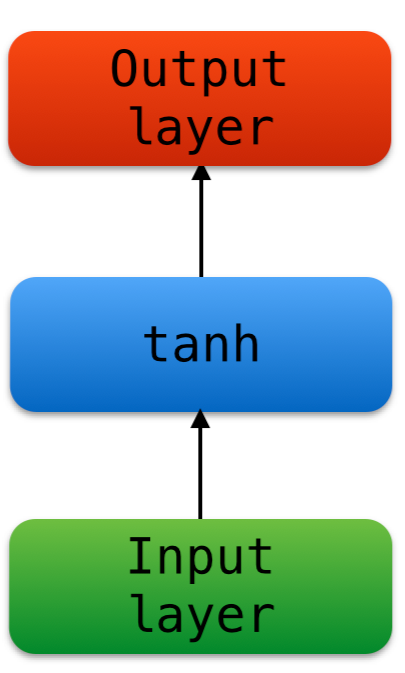
\includegraphics[width=0.22\columnwidth]{images/simRNN.png}
} %
\subfigure[1-layer GRU-RNN]{\label{fig:1GRU}
\centering
  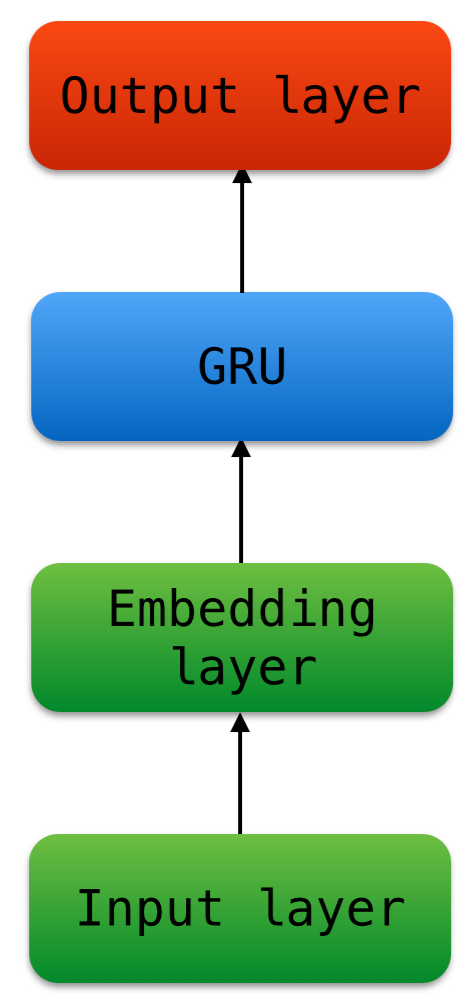
\includegraphics[width=0.22\columnwidth]{images/GRUlayer.png}
}
\subfigure[1-layer LSTM-RNN]{\label{fig:1LSTM}
\centering
  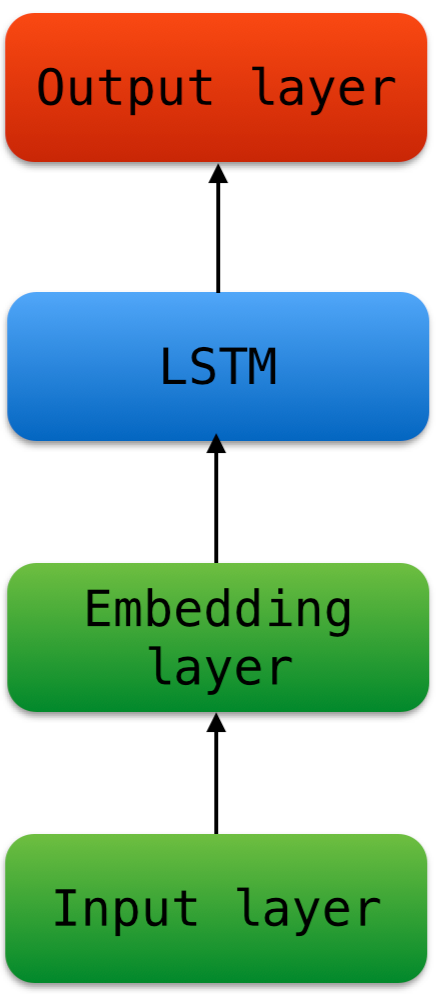
\includegraphics[width=0.22\columnwidth]{images/LSTMLayer.png}
}
\subfigure[2-layer GRU-RNN]{\label{fig:2GRU}
\centering
  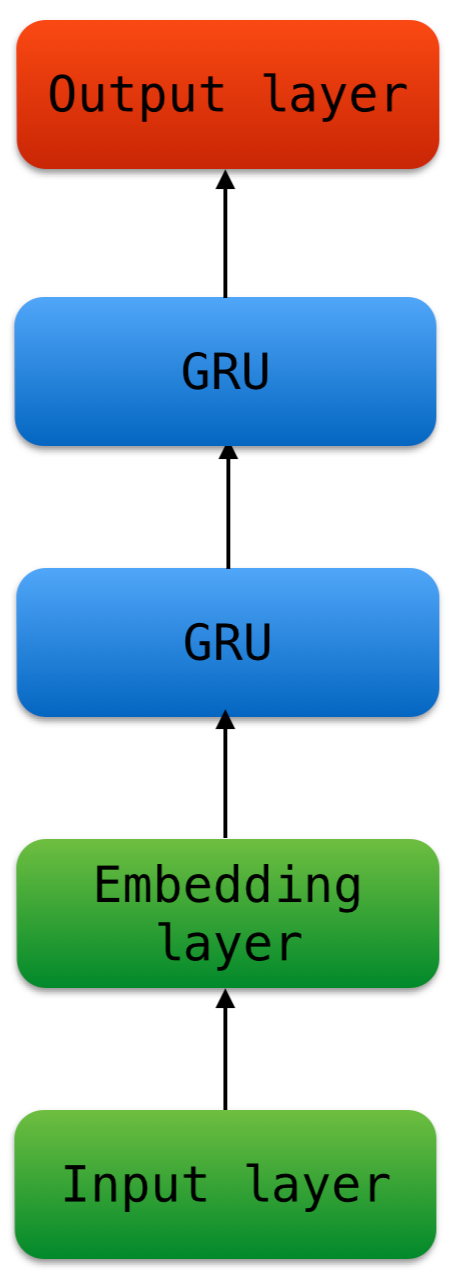
\includegraphics[width=0.22\columnwidth]{images/2gru.png}
}
\subfigure[FastText]{\label{fig:fasttext}
\centering
  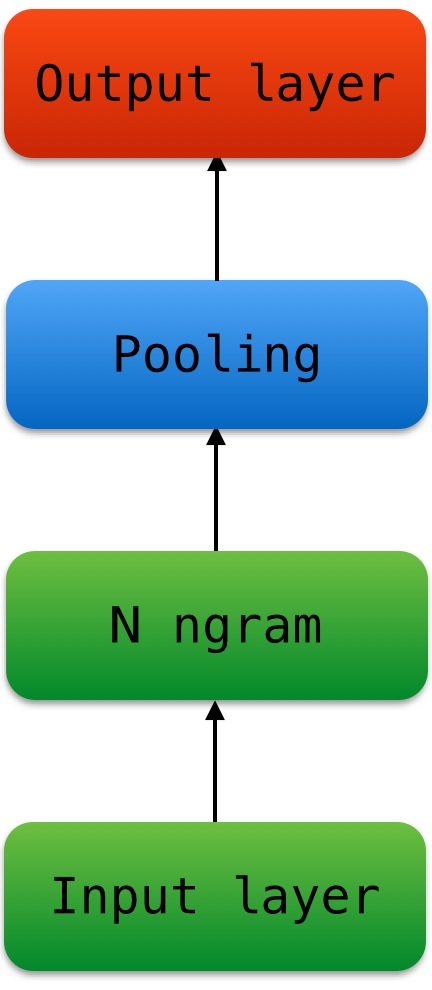
\includegraphics[width=0.22\columnwidth]{images/fasttext.png}
}
\subfigure[Hybrid CNN + LSTM (C-LSTM)]{\label{fig:CNNLSTM}
\centering
  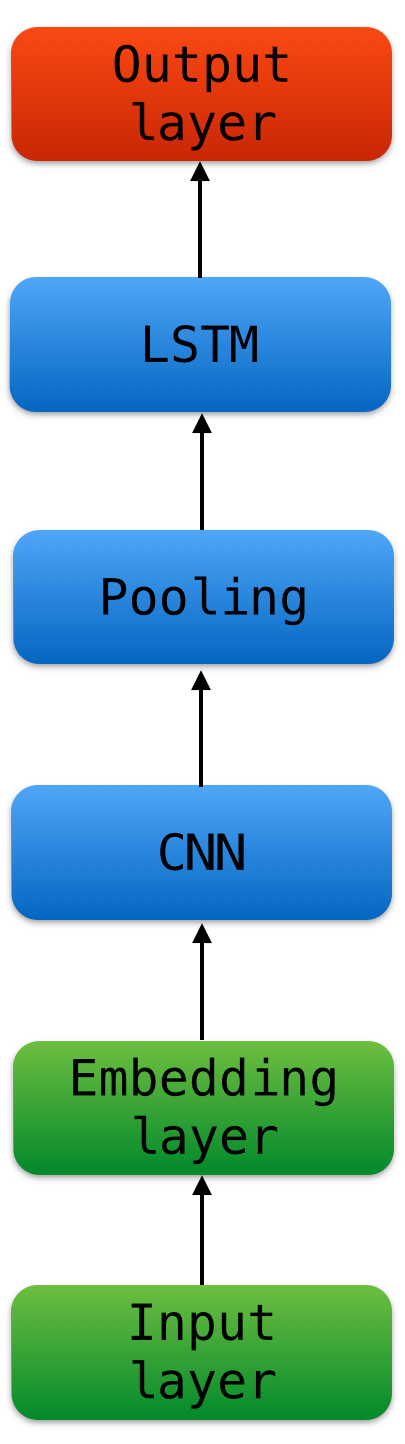
\includegraphics[width=0.22\columnwidth]{images/CNNLSTM.png}
}
\caption{neural network model for single tweet classification 1}
\label{fig:NNModel1}
\end{figure}



  \subsection{Data Preparing} % (fold)
We test the above models with same dataset and same shuffled sequence as the RF, SVM model. The difference is the we feed only the text of each tweet to the neural network models. And we randomly take 20\% data from the training set to be the valid set for optimizing the parameters. 
 \subsection{Embedding Layer}  
 The first layer is embedding layer which is set up the same to all models.The embedding size is 50. The output of the embedding layer is the vectors presenting the words.  
  \subsection{Tested Results}  
  The best accuracy result is C-LSTM model as shown in table \ref{tab:single_result2}. To avoid overfitting we use 10-fold cross validation and dropout technology.  
  
 \begin{table*}[!h]
 \centering
\scalebox{1.1}{
 \begin{tabular}{@{}lllllll@{}}
 \toprule
 \textbf{Model} & \textbf{Accuracy} \\ \midrule
 CNN+RNN & \textbf{0.8119 }\\
 2-layer GRU & 0.7891\\
 GRU & 0.7644\\
 LSTM & 0.7493\\
 Basic RNN with tanh &  0.7291\\
 FastText &  0.6602\\ \bottomrule
 \end{tabular}}
 \caption{Prediction Accuracy of Different Single Tweet's Creditability Scoring Models }
 \label{tab:single_result2}
\end{table*}

\newpage
  \subsection{CNN + LSTM (C-LSTM) Model}  
  The best accuracy result is C-LSTM model which is invented by zhou \cite{zhou2015c}. The architecture of the model is shown in figure \ref{fig:CNNLSTMde}. Front hidden layer is a CNN which can split the text to different features and the pooling layer group the same type of feature together then the last hidden layer is a LSTM layer. According to his paper C-LSTM achieved the best result for a 2-classification task with 87.8\% accuracy. And in our test it gets 81\% accuracy. 
  
  \begin{figure}
\centering
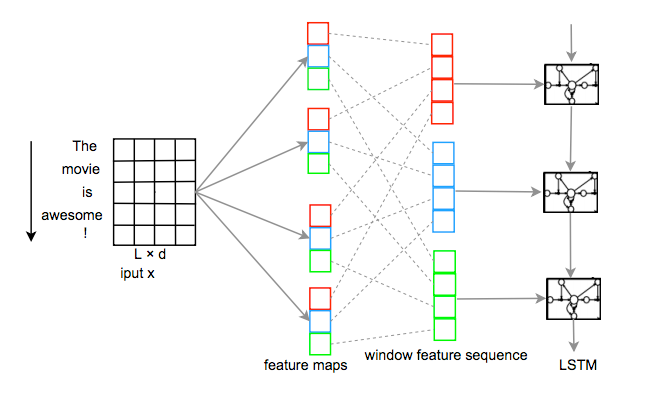
\includegraphics[width=0.8\columnwidth]{images/CNNLSTMdetail.png}
\caption{The architecture of C-LSTM Interface (source: \cite{zhou2015c})}
\label{fig:CNNLSTMde}
\end{figure} 
